\documentclass[tikz]{standalone}
\usepackage{amsmath}
\usepackage{amssymb}
\usepackage{braket}
\usepackage{tikz,tkz-euclide}
\usetikzlibrary{arrows,calc,patterns}

\begin{document}
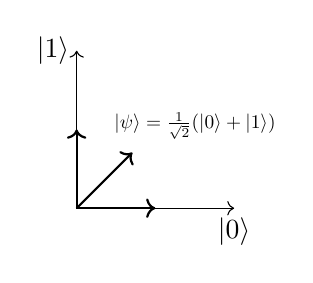
\begin{tikzpicture}
    \draw [<->] (0,2) -- (0, 0) -- (2, 0);
    \node at (2, -0.3) {$\ket{0}$};
    \node at (-0.3, 2) {$\ket{1}$};
    \draw [->,thick] (0, 0) -- (45:1);
    \draw [->,thick] (0, 0) -- (0, 1);
    \draw [->,thick] (0, 0) -- (1, 0);
    \node[anchor=south west] at (70:0.8) {\scalebox{0.7}{ 
        $\ket{\psi}=\frac{1}{\sqrt{2}}(\ket{0}+\ket{1})$}};
\end{tikzpicture}
\end{document}
